\documentclass{standalone}
\author{Quinten Bruynseraede}
\usepackage{tikz}
\usetikzlibrary{shapes}
\title{Tikz grafen}
\begin{document}\pagestyle{empty}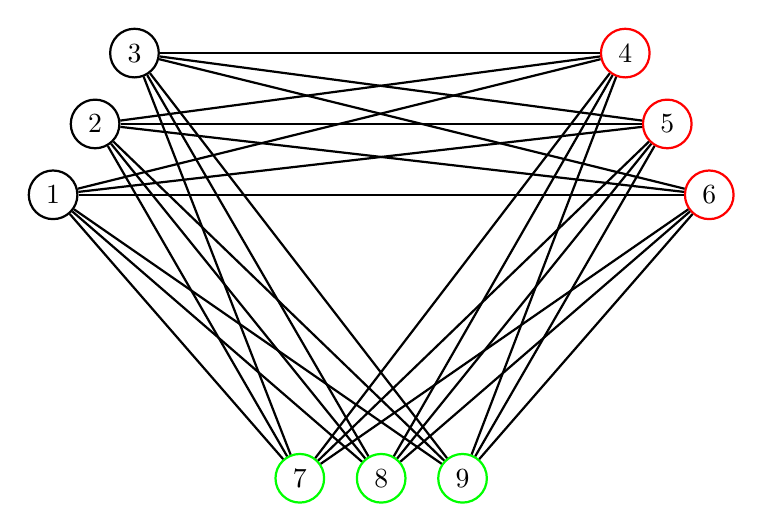
\begin{tikzpicture}\node[shape=circle,draw=black,align=center,line width=0.8pt] (0) at (4.666666666666667,13.966666666666667) {3};
\node[shape=circle,draw=black,align=center,line width=0.8pt] (1) at (4.166666666666667,13.066666666666666) {2};
\node[shape=circle,draw=black,align=center,line width=0.8pt] (2) at (3.6333333333333333,12.166666666666666) {1};
\node[shape=circle,draw=red,align=center,line width=0.8pt] (3) at (10.9,13.966666666666667) {4};
\node[shape=circle,draw=red,align=center,line width=0.8pt] (4) at (11.433333333333334,13.066666666666666) {5};
\node[shape=circle,draw=red,align=center,line width=0.8pt] (5) at (11.966666666666667,12.166666666666666) {6};
\node[shape=circle,draw=green,align=center,line width=0.8pt] (6) at (6.766666666666667,8.566666666666666) {7};
\node[shape=circle,draw=green,align=center,line width=0.8pt] (7) at (7.8,8.566666666666666) {8};
\node[shape=circle,draw=green,align=center,line width=0.8pt] (8) at (8.833333333333334,8.566666666666666) {9};

\path [-,draw=black,line width=0.8pt] (0) edge node {} (3);
\path [-,draw=black,line width=0.8pt] (0) edge node {} (4);
\path [-,draw=black,line width=0.8pt] (0) edge node {} (5);
\path [-,draw=black,line width=0.8pt] (0) edge node {} (8);
\path [-,draw=black,line width=0.8pt] (0) edge node {} (7);
\path [-,draw=black,line width=0.8pt] (0) edge node {} (6);
\path [-,draw=black,line width=0.8pt] (1) edge node {} (3);
\path [-,draw=black,line width=0.8pt] (1) edge node {} (4);
\path [-,draw=black,line width=0.8pt] (1) edge node {} (5);
\path [-,draw=black,line width=0.8pt] (2) edge node {} (8);
\path [-,draw=black,line width=0.8pt] (2) edge node {} (7);
\path [-,draw=black,line width=0.8pt] (2) edge node {} (6);
\path [-,draw=black,line width=0.8pt] (3) edge node {} (6);
\path [-,draw=black,line width=0.8pt] (3) edge node {} (7);
\path [-,draw=black,line width=0.8pt] (3) edge node {} (8);
\path [-,draw=black,line width=0.8pt] (4) edge node {} (6);
\path [-,draw=black,line width=0.8pt] (3) edge node {} (2);
\path [-,draw=black,line width=0.8pt] (4) edge node {} (2);
\path [-,draw=black,line width=0.8pt] (4) edge node {} (7);
\path [-,draw=black,line width=0.8pt] (4) edge node {} (8);
\path [-,draw=black,line width=0.8pt] (5) edge node {} (2);
\path [-,draw=black,line width=0.8pt] (5) edge node {} (6);
\path [-,draw=black,line width=0.8pt] (5) edge node {} (7);
\path [-,draw=black,line width=0.8pt] (5) edge node {} (8);
\path [-,draw=black,line width=0.8pt] (1) edge node {} (6);
\path [-,draw=black,line width=0.8pt] (1) edge node {} (7);
\path [-,draw=black,line width=0.8pt] (1) edge node {} (8);
\end{tikzpicture}
\end{document}